\documentclass[border=5pt]{standalone}

\usepackage[utf8]{inputenc}
\usepackage{garamondx}

\usepackage[x11names]{xcolor}

\definecolor{darkolivegreen}{rgb}{0.33, 0.42, 0.18}
\definecolor{darkbyzantium}{rgb}{0.36, 0.22, 0.33}
\definecolor{darkelectricblue}{rgb}{0.33, 0.41, 0.47}
\definecolor{deepchestnut}{rgb}{0.73, 0.31, 0.28}

\usepackage{tikz}
\usetikzlibrary{shapes.geometric, arrows, positioning}

\tikzstyle{required}=[rectangle, rounded corners, minimum width=7em, minimum height=2em, text centered, draw=black, fill=darkolivegreen!30, text width=7em]
\tikzstyle{questions} = [rectangle, rounded corners, minimum width=7em, minimum height=2em, text centered, draw=black, fill=darkbyzantium!30, text width=7em]
\tikzstyle{process}=[rectangle, rounded corners, minimum width=10em, minimum height=2em, text centered, draw=black, fill=darkelectricblue!30, text width=7em]
\tikzstyle{demo}=[rectangle, rounded corners, minimum width=7em, minimum height=2em, text centered, draw=black, fill=deepchestnut!30, text width=7em]
\tikzstyle{arrow}=[very thick, ->, >=latex]

\begin{document}
	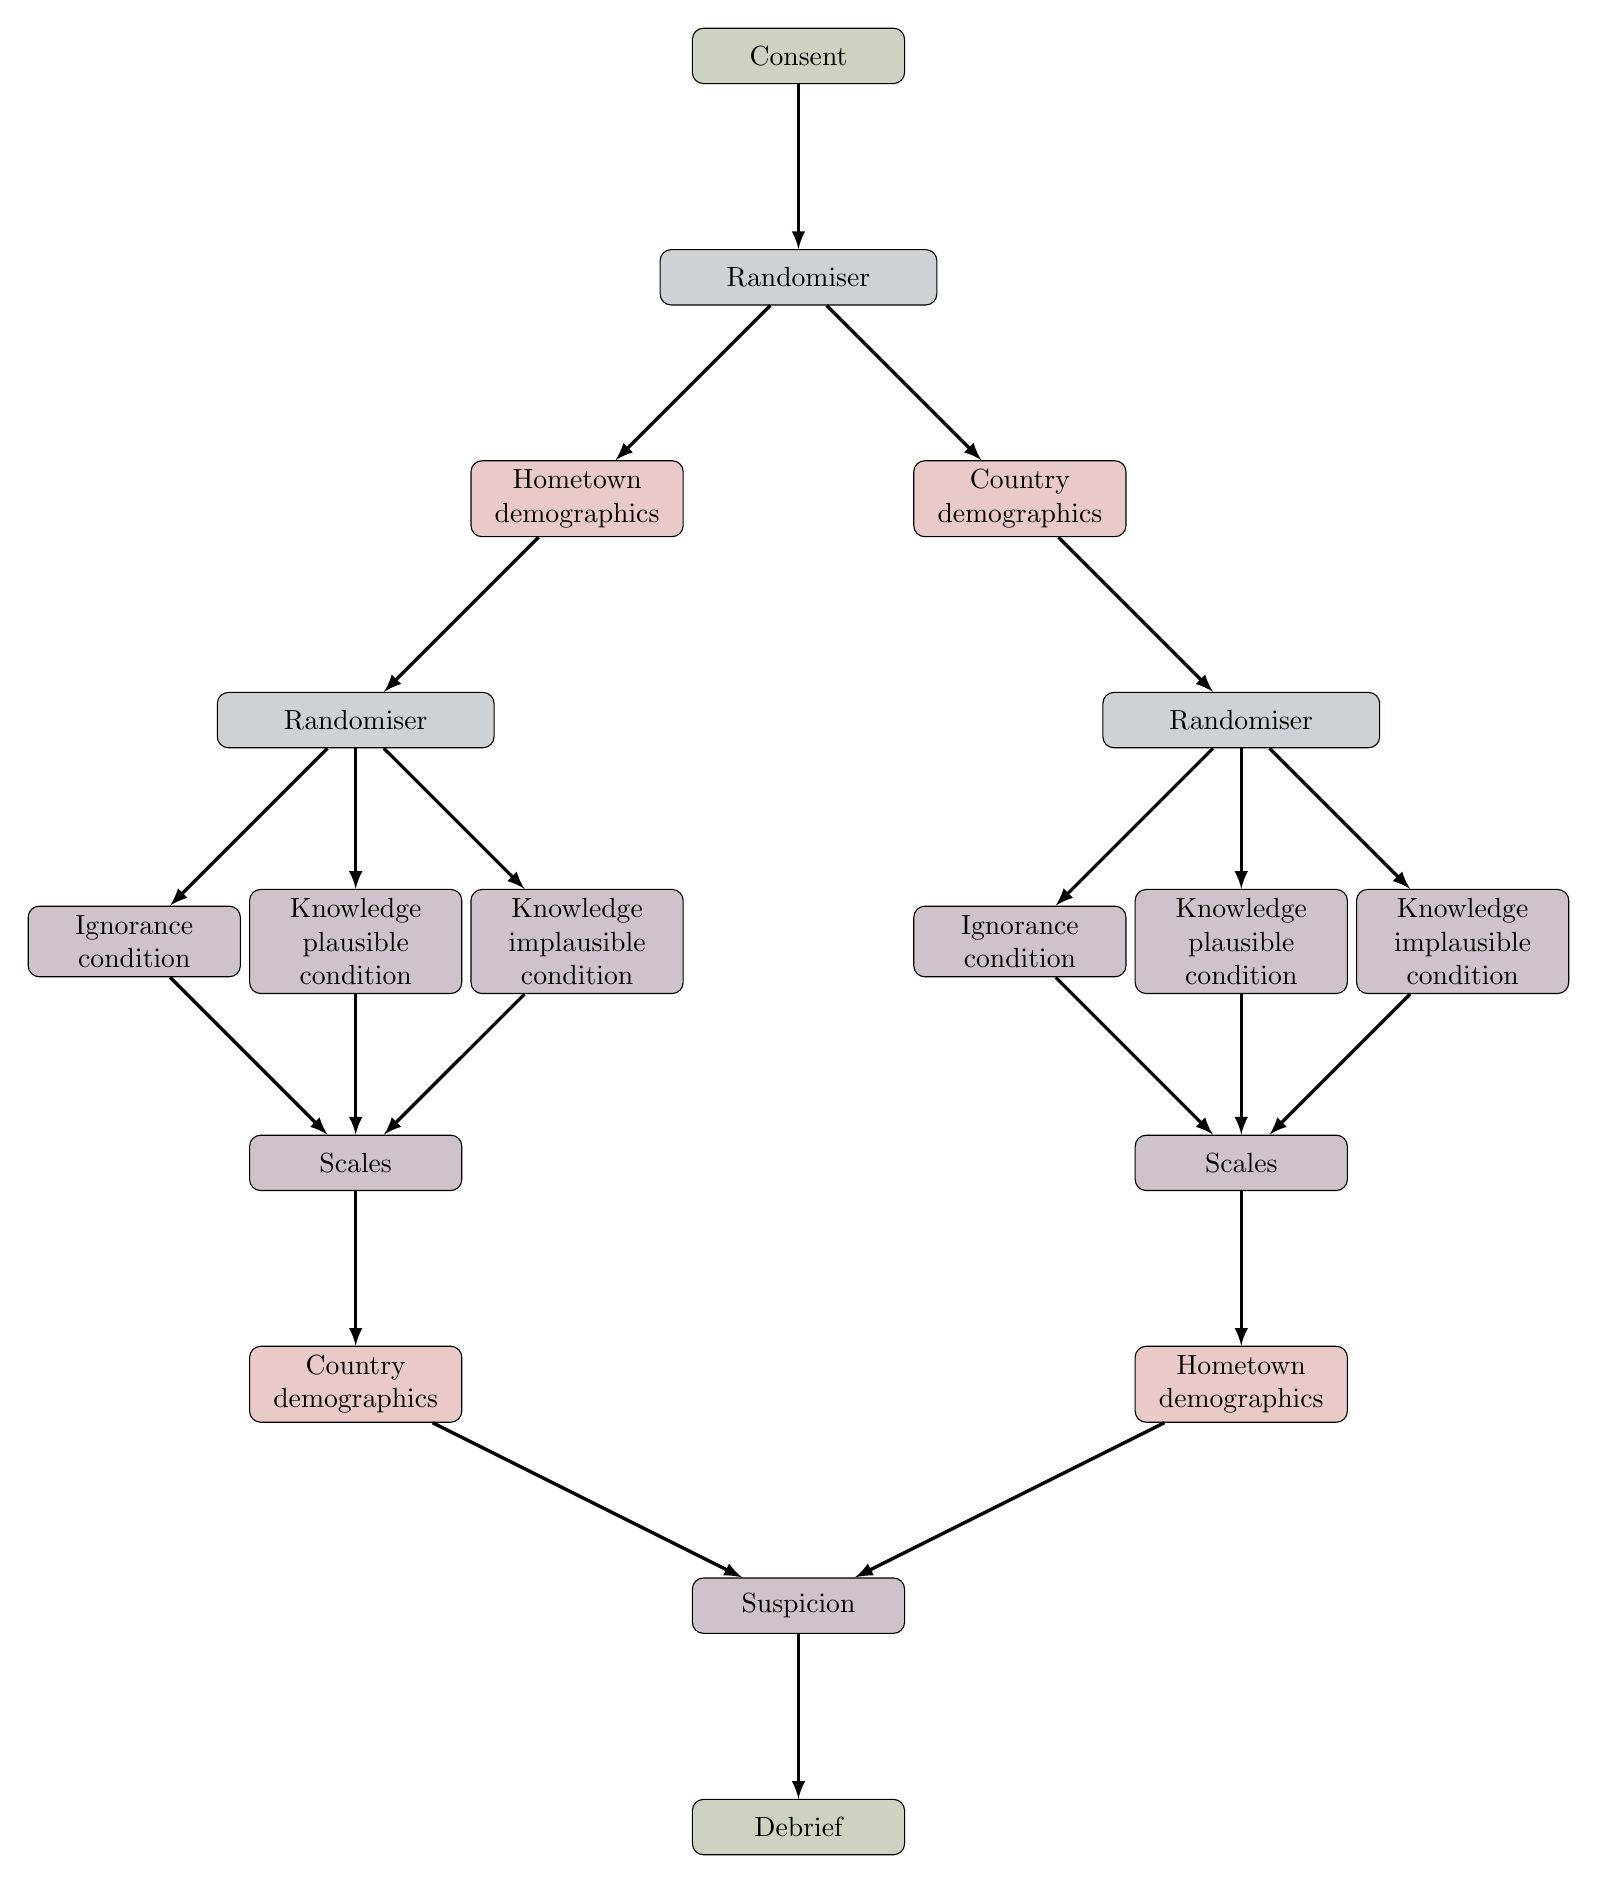
\begin{tikzpicture}[node distance=8em]		
		\node(n1)[required]{Consent};
		\node(n1-5)[below of=n1,process]{Randomiser};
		\node(n1-1)[below of=n1-5]{};
		\node(n2-1)[demo,left of=n1-1]{Hometown demographics};
		\node(n2-2)[demo,right of=n1-1]{Country demographics};
		\node(n2-1-1)[below of=n2-1]{};
		\node(n2-2-1)[below of=n2-2]{};
		\node(n3-1)[process,left of=n2-1-1]{Randomiser};
		\node(n3-2)[process,right of=n2-2-1]{Randomiser};
		\node(n3-1-1)[below of=n3-1]{};
		\node(n3-2-1)[below of=n3-2]{};
		\node(n4-1-1)[questions,left of=n3-1-1]{Ignorance condition};
		\node(n4-1-2)[questions,below of=n3-1]{Knowledge plausible condition};
		\node(n4-1-3)[questions,right of=n3-1-1]{Knowledge implausible condition};
		\node(n4-2-1)[questions,left of=n3-2-1]{Ignorance condition};
		\node(n4-2-2)[questions,below of=n3-2]{Knowledge plausible condition};
		\node(n4-2-3)[questions,right of=n3-2-1]{Knowledge implausible condition};
		\node(n5-1)[questions,below of=n4-1-2]{Scales};
		\node(n5-2)[questions,below of=n4-2-2]{Scales};
		\node(n6-1)[demo,below of=n5-1]{Country demographics};
		\node(n6-2)[demo,below of=n5-2]{Hometown demographics};
		\node(n7-1)[below of=n6-1]{};
		\node(n7-2)[right of=n7-1]{};
		\node(n7-3)[questions,right of=n7-2]{Suspicion};
		\node(n8)[required,below of=n7-3]{Debrief};
		
		\draw[arrow](n1)--(n1-5);
		\draw[arrow](n1-5)--(n2-1);
		\draw[arrow](n1-5)--(n2-2);
		\draw[arrow](n2-1)--(n3-1);
		\draw[arrow](n2-2)--(n3-2);
		\draw[arrow](n3-1)--(n4-1-1);
		\draw[arrow](n3-1)--(n4-1-2);
		\draw[arrow](n3-1)--(n4-1-3);
		\draw[arrow](n3-2)--(n4-2-1);
		\draw[arrow](n3-2)--(n4-2-2);
		\draw[arrow](n3-2)--(n4-2-3);
		\draw[arrow](n4-1-1)--(n5-1);
		\draw[arrow](n4-1-2)--(n5-1);
		\draw[arrow](n4-1-3)--(n5-1);
		\draw[arrow](n4-2-1)--(n5-2);
		\draw[arrow](n4-2-2)--(n5-2);
		\draw[arrow](n4-2-3)--(n5-2);
		\draw[arrow](n5-1)--(n6-1);
		\draw[arrow](n5-2)--(n6-2);
		\draw[arrow](n6-1)--(n7-3);
		\draw[arrow](n6-2)--(n7-3);
		\draw[arrow](n7-3)--(n8);
	\end{tikzpicture}
\end{document}